\begin{figure} [!ht]
\begin{center}
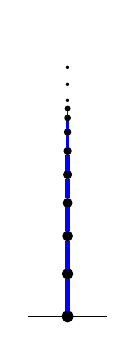
\begin{tikzpicture}
	\begin{scope} [every node/.style={scale=0.3, style=circle, draw, fill=black}]
		\node [scale=1.4] (1) at (0, -1.80){};
		\node [scale=1.3] (2) at (0, -1.26){};
		\node [scale=1.2] (3) at (0, -0.78){};
		\node [scale=1.1] (4) at (0, -0.36){};
		\node [scale=1]   (5) at (0, 0)      {};
		\node [scale=0.9] (6) at (0, 0.3)  {};
		\node [scale=0.8] (7) at (0, 0.54) {};
		\node [scale=0.7] (8) at (0, 0.72) {};
		\node [scale=0.6] (9) at (0, 0.84) {};
		\node [scale=0.2, fill=white, draw=none] at (0, 1.1) {$\vdots$};
	\end{scope}
	\draw (-0.5,-1.80) -- (0.5, -1.80);
	\draw[blue, ultra thick] (1)--(2);
	\draw[blue, ultra thick] (2)--(3);
	\draw[blue, ultra thick] (3)--(4);
	\draw[blue, ultra thick] (4)--(5);
	\draw[blue, ultra thick] (5)--(6);
	\draw[blue, thick] (6)--(7);
	\draw[blue, thick] (7)--(8);
	\draw[blue] (8)--(9);
	\node[scale=1.5] at (0, 1.3) {\scriptsize$\vdots$};
\end{tikzpicture}
\end{center}
\caption{The first infinite game}
\end{figure}